\documentclass[a4paper,11pt]{article}
\usepackage[left=2cm,text={17cm, 24cm},top=3cm]{geometry}
\usepackage{times}
\usepackage[czech]{babel}
\usepackage[utf8]{inputenc}
\usepackage[IL2]{fontenc}
\usepackage{multirow}
\usepackage[ruled,longend,czech]{algorithm2e}
\usepackage{graphics}
\usepackage{lscape}
\usepackage{picture}
\usepackage[ampersand]{easylist}
\newcommand{\myuv}[1]{\quotedblbase #1\textquotedblleft}
\usepackage{enumitem}
\setlist[enumerate]{label*=\arabic*.}

\usepackage{array}
\newcolumntype{L}[1]{>{\raggedright\let\newline\\\arraybackslash\hspace{0pt}}m{#1}}
\newcolumntype{C}[1]{>{\centering\let\newline\\\arraybackslash\hspace{0pt}}m{#1}}
\newcolumntype{R}[1]{>{\raggedleft\let\newline\\\arraybackslash\hspace{0pt}}m{#1}}

\begin{document}
    \begin{titlepage}
	\begin{center}
	    {\Huge\textsc{Vysoké učení technické v~Brně\\}}
	    {\huge\textsc{Fakulta informačních technologií\\}}
	    \vspace{\stretch{0.382}}
	    {\LARGE AIS -- projekt\\}
	    \medskip
	    {\LARGE Prvotní analýza a plán projektu\\}
	    \medskip
	    {\Huge Evidence výpočetní techniky}
	\end{center}
	\vspace{\stretch{0.618}}
	{\Large \hfill Klimaj Daniel}

	{\Large \today \hfill Svoboda Ondřej}

	{\Large \hfill Večeřa Vojtěch} 
    \end{titlepage} 

    \section*{Neformální specifikace}

    Je zapotřebí vytvořit nový modul informačního systému FIT, sloužící k evidenci výpočetní techniky. Systém musím zajišťovat komplexní správu veškeré výpočetní techniky v areálu FIT VUT.

    V FIT VUT se nachází velká řada výpočetní techniky, kterou je nutné evidovat. Evidován musí být každý kus samostatně a to i oddělitelné a vyměnitelné součástky počítačů jako např. pevné disky, grafické karty atd. U každého kusu techniky je nutné znát jeho výrobce, model a jeho stav, který udává, zda je zařízení v pořádku, je rozbité atd. Dále by mělo být možné u zařízení specifikovat další dodatečné informace.

    Na FIT pracují zaměstnanci, kteří mohou jednotlivé kusy výpočetní techniky vlastnit. V systému musí být možné každému zaměstnanci specifikovat jeho práva v rámci systému. Každý kus techniky může současně vlastnit pouze jediný zaměstnanec. Zaměstnanec může také žádat o přesun techniky mezi jednotlivými místnostmi. V takovém případě musí uvést ID zařízení, důvod přesunu a odkud kam požaduje techniku přesunout. Uchovávaný je také čas žádosti a zda již byl přesun proveden. Další možnou akcí zaměstnance je nahlásit poruchu zařízení servisnímu technikovi. Ten se stará o opravu zařízení a do IS zadává záznam o této opravě a může také vyhledávat v seznamu vad. Další kategorií zaměstnanců je tzv. materiálový koordinátor. Jeho úkolem je správa všech zařízení, jejich vkládání, úprava a vyjímání ze systému. Stará se také o seznam místností a schvaluje přesuny techniky. Informační systém by měl také obsahovat roli personalisty. Ten se stará o správu všech uživatelů v systému tzn. jejich přidávání, mazání a upravování. Stejné úkony může provádět i s odděleními. Každý zaměstnanec náleží nějakému oddělení a každé oddělení má svého vedoucího z řad zaměstnanců. 

    O každém zaměstnanci musí systém znát jeho login, jméno, příjmení, datum narození, mail, mobilní číslo a telefonní číslo do kanceláře. Je také nutné uchovávat heslo, s kterým se zaměstnanec přihlašuje do systému.

    Dále je nutné v systému uchovávat seznam místností na FIT. Místnosti mohou být dvou typů a to buď učebna nebo kancelář. Každý zaměstnanec sídlí v nějaké kanceláři. U každé místnosti je nutné znát její polohu, tzn.~např.~patro, křídlo budovy, kde se nachází, a dále její rozměry. U učeben je nutné znát počet míst k sezení, počet řad a míst na řadu. U kanceláří je nutné znát počet elektrických a ethernetových zásuvek, protože od toho se může odvozovat přidělování techniky do jednotlivých kanceláří. Každé zařízení může být v jeden okamžik jen v jedné místnosti a každá místnost přísluší jednomu oddělení.

    Každý zaměstnanec by měl mít možnost zobrazit si vybavení dané učebny. Materiálový koordinátor si může u každého zaměstnance zobrazit seznam techniky, která mu patří a také filtrovat zařízení dle jejich typu atd. 

    Systém bude fungovat jako modul již funkčního informačního systému. Bude se dotazovat databázového serveru od kterého bude následně dostávat požadované odpovědi. Vzhledem k pravděpodobnému velkému množství zpracovávaných položek musí být systém co nejpřehlednější a intuitivní. 

    \section*{Analýza požadavků}

    Dle neformální specifikace bylo možné sestavit tyto požadavky:

    \begin{easylist}
	\ListProperties(Hide=100, Hang=true, Progressive=3ex, Style*=-- ,Style2*=$\bullet$ )
	& abstraktní aktéři:
	&& Zaměstanec -- jedná se o nejobecnějšího uživatele systému. Zahrnuje akce, které může podnikat každý zaměstnanec FIT VUT. Konkrétním potomkem je aktér ze skupiny Ostatní zaměstnanci.
	& speciální aktéři:
	&& Personalista -- je aktér, který komunikuje se všemi případy užití, které se zabývají správou uživatelů a oddělení.
	&& Technik VT -- reprezentuje aktéra, který se stará o správu oprav jednotlivých technických zařízení.
	&& Materiálový koordinátor -- je aktér, který má na starost správu všech zařízení, učeben a přesunů.

    \end{easylist}

    \noindent
    Díky dědičnosti bylo možné sloučit společné případy užití jednomu aktérovi.

    \begin{figure}[ht]
	\begin{center}
	    \scalebox{0.7}{
		\includegraphics{img/3_iterace.pdf}
	    } 
	\end{center}
	\caption{Digram zobrazuje jednotlivé aktéry s jejich příslušnými případy užití.}
	\label{pic1} 
    \end{figure}

    \section*{Plán projektu}

    Dle analýzy požadavků lze odvozovat, že realizaci výsledného systému je nutné rozdělit do několika iterací, které se použijí při iterativním životním cyklu. Z obrázku \ref{pic1} lze usuzovat, že bude nejlepší použít tři iterace, kde v každé iteraci přidáme jednoho speciálního aktéra. V první iteraci se budeme zabývat personalistou, v druhé materiálovým koordinátorem a ve třetí technikem. Tím nám tedy vznikne realizace celého informačního systému. 

    \newpage
    \subsection*{1. iterace}

    \begin{figure}[ht]
	\begin{center}
	    \scalebox{0.7}{
		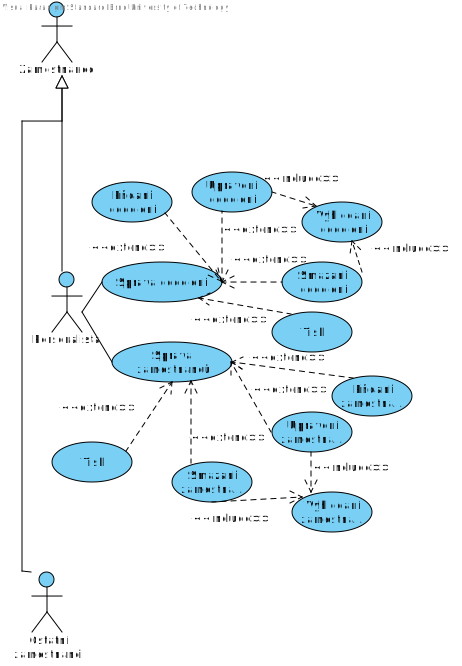
\includegraphics{img/1_iterace.pdf}
	    } 
	\end{center}
	\caption{Po první iteraci by mělo být možné vkládat do systému nové uživatele, uživatele odebírat a upravovat. Za tímto účelem bude v první iteraci již figurovat personalista.}
	\label{pic2} 
    \end{figure}

    \newpage
    \subsection*{2. iterace}

    \begin{figure}[ht]
	\begin{center}
	    \scalebox{0.7}{
		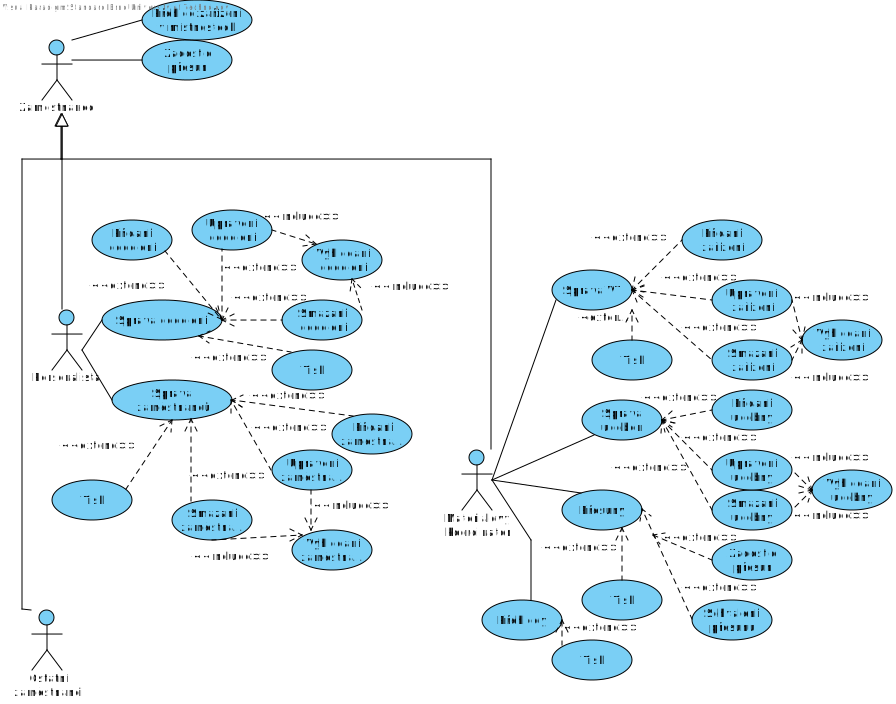
\includegraphics{img/2_iterace.pdf}
	    } 
	\end{center}
	\caption{Ve druhé iteraci přidáme materiálového koordinátora a tím umožníme do systému vkládat nové kusy techniky. Rozšíří se také případy užití všech zaměstnanců.}
	\label{pic3} 
    \end{figure}

    \newpage
    \subsection*{3. iterace}

    \begin{figure}[ht]
	\begin{center}
	    \scalebox{0.7}{
		\includegraphics{img/3_iterace.pdf}
	    } 
	\end{center}
	\caption{Nakonec systém rozšíříme o správu jednotlivých poruch a s tím přidáme i podporu pro technika VT. Tímto se zkompletuje celý systém a aplikace bude hotová.}
	\label{pic4} 
    \end{figure}

    \begin{table}[ht]
	\centering
	\label{my-label}
	\begin{tabular}{|R{0.2\textwidth}|L{0.8\textwidth}|}
	    \hline
	    ID: & 1 \\ \hline
	    Název: & \textbf{Přidej zaměstnance} \\ \hline
	    Vytvořeno: & Ondřej Svoboda \\ \hline
	    Popis: & Personalista přidá zaměstnance do systému \\ \hline
	    Primární aktéři: & Personalista \\ \hline
	    Sekundární aktéři: & \\ \hline
	    Předpoklady: & Personalista je autorizován v systému a má práva na vkládání nových zaměstnanců \\ \hline
	    \begin{tabular}[c]{@{}r@{}}Následné\\ podmínky:\end{tabular} & Nový zaměstnanec je přidán do systému \\ \hline
		Akce pro spuštění: & Personalista vybere "Přidat zaměstnance" \\ \hline
	    Hlavní tok: & \begin{minipage}[t]{\linewidth}
		\begin{enumerate}[nosep, after=\strut, leftmargin=20pt]
		    \item Systém nabídne personalistovi zadání údajů o zaměstnanci
		    \item Dokud nejsou správně zadány údaje o zaměstnanci
			\begin{enumerate}[nosep, after=\strut, leftmargin=20pt]
			    \item Personalista zadá zaměstnanci jeho unikátní login
			    \item Personalista zadá rodné číslo, jméno, příjmení, datum narození nového zaměstnance
			    \item Personalista zadá mobilní číslo, číslo do kanceláře a mail nového zaměstnance
			    \item Personalista potvrdí zadané hodnoty
			\end{enumerate} 
		    \item Systém vygeneruje uživateli nové heslo
		    \item Systém zaznamená nového zaměstnance
		\end{enumerate} 
	    \end{minipage}\\ \hline
	    Alternativní toky: & \begin{tabular}[c]{@{}l@{}}Uživatel již v systému existuje\\ Nebyly vyplněny povinné údaje\end{tabular} \\ \hline
		Vyjímky: & \begin{tabular}[c]{@{}l@{}}Storno\\ Selhání operace\\ Selhání systému\end{tabular} \\ \hline
		    Frekvence: & Méně často \\ \hline

	\end{tabular}
    \end{table}

    \begin{table}[ht]
	\centering
	\label{my-label}
	\begin{tabular}{|R{0.2\textwidth}|L{0.8\textwidth}|}
	    \hline
	    ID: & 1.1 \\ \hline
	    Název: & \textbf{Přidej zaměstnance: zaměstnanec již existuje} \\ \hline
	    Vytvořeno: & Ondřej Svoboda \\ \hline
	    Popis: & Systém informuje personalistu, že daný zaměstnanec je již v systému \\ \hline
	    Primární aktéři: & Personalista \\ \hline
	    Sekundární aktéři: & \\ \hline
	    Předpoklady: & Personalista zadal o novém zaměstnanci jméno, příjmení, rodné číslo a datum narození takové, že se všechny tyto údaje shodují s jiným jedním zaměstnancem v systému \\ \hline
	    \begin{tabular}[c]{@{}r@{}}Následné \\ podmínky:\end{tabular} & Je zobrazeno upozornění, že zaměstnanec již existuje v systému \\ \hline
		Akce pro spuštění: & Personalista v kroku 2.5 potvrdí vložení zaměstnance s platným předpokladem \\ \hline
	    Alternativní tok: & \begin{minipage}[t]{\linewidth}
		\begin{enumerate}[nosep, after=\strut, leftmargin=20pt]
		    \item Systém informuje uživatele, že se snaží vložit již vloženého zaměstnance
		    \item Návrat k bodu 2 hlavního toku
		\end{enumerate} 
	    \end{minipage} \\ \hline
	    Frekvence: & zřídka \\ \hline
	\end{tabular}
    \end{table}

    \begin{table}[ht]
	\centering
	\label{my-label}
	\begin{tabular}{|R{0.2\textwidth}|L{0.8\textwidth}|}
	    \hline
	    ID: & 1.2 \\ \hline
	    Název: & \textbf{Přidej zaměstnance: nebyly vyplněny povinné údaje} \\ \hline
	    Vytvořeno: & Ondřej Svoboda \\ \hline
	    Popis: & Systém informuje personalistu, že nevyplnil nějaký povinný údaj \\ \hline
	    Primární aktéři: & Personalista \\ \hline
	    Sekundární aktéři: & \\ \hline
	    Předpoklady: & Personalista nezadal login, jméno, příjmení, rodné č., datum narození, mobilní č., číslo do kanceláře nebo mail nového zaměstnance.\\ \hline
	    \begin{tabular}[c]{@{}r@{}}Následné \\ podmínky:\end{tabular} & Je zobrazeno upozornění, že nějaký povinný údaj je nevyplněn \\ \hline
		Akce pro spuštění: & Personalista v kroku 2.5 potvrdí vložení zaměstnance s platným předpokladem \\ \hline
	    Alternativní tok: & \begin{minipage}[t]{\linewidth}
		\begin{enumerate}[nosep, after=\strut, leftmargin=20pt]
		    \item Systém informuje uživatele, že se není vyplněn povinný údaj
		    \item Návrat k bodu 2 hlavního toku
		\end{enumerate} 
	    \end{minipage}\\ \hline
	    Frekvence: & zřídka \\ \hline
	\end{tabular}
    \end{table}

    \begin{table}[ht]
	\centering
	\label{my-label}
	\begin{tabular}{|R{0.2\textwidth}|L{0.8\textwidth}|}
	    \hline
	    ID: & 1.E.1 \\ \hline
	    Název: & \textbf{Přidej zaměstnance: Storno} \\ \hline
	    Vytvořeno: & Ondřej Svoboda \\ \hline
	    Popis: & Personalista ukončil případ užití \\ \hline
	    Primární aktéři: & Personalista \\ \hline
	    Sekundární aktéři: & \\ \hline
	    Předpoklady: & \\ \hline
	    \begin{tabular}[c]{@{}r@{}}Následné\\ podmínky:\end{tabular} & Nový zaměstnanec nebyl přidán do systému \\ \hline
		Akce pro spuštění: & Personalista zadal storno během průběhu hlavního toku \\ \hline
	    Tok: & Návrat na místo odkud byl vyvolán případ užití \\ \hline
	    Frekvence: & Zřídka \\ \hline
	\end{tabular}
    \end{table}

    \begin{table}[ht]
	\centering
	\label{my-label}
	\begin{tabular}{|R{0.2\textwidth}|L{0.8\textwidth}|}
	    \hline
	    ID: & 1.E.2 \\ \hline
	    Název: & \textbf{Přidej zaměstnance: Selhání operace} \\ \hline
	    Vytvořeno: & Ondřej Svoboda \\ \hline
	    Popis: & Systém nedokáže dokončit průběh operace \\ \hline
	    Primární aktéři: & Personalista, systém \\ \hline
	    Sekundární aktéři: & \\ \hline
	    Předpoklady: & \begin{tabular}[c]{@{}l@{}}Systému se nepodařilo provést nějaký krok hlavního toku\\Systém stále funguje korektně\end{tabular} \\ \hline
		\begin{tabular}[c]{@{}r@{}}Následné\\ podmínky:\end{tabular} & Nový zaměstnanec nebyl přidán do systému \\ \hline
		    Akce pro spuštění: & Selhání v průběhu hlavního toku \\ \hline
	    Tok: & \begin{minipage}[t]{\linewidth}
		\begin{enumerate}[nosep, after=\strut, leftmargin=20pt]
		    \item Personalista je informován o selhání případu užití
		    \item Návrat na místo odkud byl vyvolán případ užití
		\end{enumerate} 
	    \end{minipage}\\ \hline
	    Frekvence: & Zřídka \\ \hline
	\end{tabular}
    \end{table}

    \begin{table}[ht]
	\centering
	\label{my-label}
	\begin{tabular}{|R{0.2\textwidth}|L{0.8\textwidth}|}
	    \hline
	    ID: & 1.E.3 \\ \hline
	    Název: & \textbf{Přidej zaměstnance: Selhání systému} \\ \hline
	    Vytvořeno: & Ondřej Svoboda \\ \hline
	    Popis: & Systém nedokáže korektně fungovat \\ \hline
	    Primární aktéři: & Personalista, systém \\ \hline
	    Sekundární aktéři: & \\ \hline
	    Předpoklady: & \begin{tabular}[c]{@{}l@{}}Systému se nepodařilo provést nějaký krok hlavního toku\\ Systém nefunguje korektně\end{tabular} \\ \hline
		\begin{tabular}[c]{@{}r@{}}Následné\\ podmínky:\end{tabular} & \begin{tabular}[c]{@{}l@{}}Nový zaměstnanec nebyl přidán do systému\\ Systém je ukončen\end{tabular} \\ \hline
		    Akce pro spuštění: & Selhání v průběhu hlavního toku \\ \hline
	    Tok: & \begin{minipage}[t]{\linewidth}
		\begin{enumerate}[nosep, after=\strut, leftmargin=20pt]
		    \item Personalista je informován o selhání případu užití
		    \item Systém je ukončen
		\end{enumerate} 
	    \end{minipage}\\ \hline
	    Frekvence: & Zřídka \\ \hline
	\end{tabular}
    \end{table}

    \begin{table}[]
	\centering
	\label{my-label}
	\begin{tabular}{|R{0.2\textwidth}|L{0.8\textwidth}|}
	    \hline
	    ID: & 2 \\ \hline
	    Název: & \textbf{Schválení přesunu} \\ \hline
	    Vytvořeno: & Ondřej Svoboda \\ \hline
	    Popis: & Materiálový koordinátor schválí přesun zařízení \\ \hline
	    Primární aktéři: & Materiálový koordinátor \\ \hline
	    Sekundární aktéři: & \\ \hline
	    Předpoklady: & Materiálový koordinátor je autorizován v systému a má práva schvalování přesunů \\ \hline
	    \begin{tabular}[c]{@{}r@{}}Následné\\ podmínky:\end{tabular} & Přesun je v systému označen jako schválený. \\ \hline
		Akce pro spuštění: & Materiálový koordinátor vybere "Schválit přesun" \\ \hline
	    Hlavní tok: & \begin{minipage}[t]{\linewidth}
		\begin{enumerate}[nosep, after=\strut, leftmargin=20pt]
		    \item Systém nabídne koordinátorovi seznam požadovaných přesunů
		    \item Koordinátor vybere konkrétní přesun dle jeho ID
		    \item Koordinátor schválí konkrétní přesun.
		    \item Systém zaznamená přesun jako schválený.
		\end{enumerate} 
	    \end{minipage}\\ \hline
	    Alternativní toky: & Přesun s tímto ID již byl schválen \\ \hline
	    Vyjímky: & \begin{tabular}[c]{@{}l@{}}Storno\\ Selhání operace\\ Selhání systému\end{tabular} \\ \hline
		Frekvence: & Často \\ \hline
	    Speciální požadavky: & \\ \hline
	\end{tabular}
    \end{table}

    \begin{table}[]
	\centering
	\label{my-label}
	\begin{tabular}{|R{0.2\textwidth}|L{0.8\textwidth}|}
	    \hline
	    ID: & 2.1 \\ \hline
	    Název: & \textbf{Schválení přesunu: Přesun již byl schválen} \\ \hline
	    Vytvořeno: & Ondřej Svoboda \\ \hline
	    Popis: & Systém informuje koordinátora, že se pokouší schválit již schválený přesun \\ \hline
	    Primární aktéři: & Koordinátor \\ \hline
	    Sekundární aktéři: & \\ \hline
	    Předpoklady: & Koordinátor vybere ke schválení přesun, který je již v systému schválen \\ \hline
	    \begin{tabular}[c]{@{}r@{}}Následné \\ podmínky:\end{tabular} & Je zobrazeno upozornění, že se koordinátor pokouší schválit již schválený přesun \\ \hline
		Akce pro spuštění: & Koordinátor v kroku 3 schválí již schválený přesun \\ \hline
	    Alternativní tok: & \begin{minipage}[t]{\linewidth}
		\begin{enumerate}[nosep, after=\strut, leftmargin=20pt]
		    \item Systém informuje koordinátora, že schvaluje již schválený přesun
		    \item Návrat k bodu 2 hlavního toku
		\end{enumerate} 
	    \end{minipage} \\ \hline
	    Frekvence: & zřídka \\ \hline
	\end{tabular}
    \end{table}

    \begin{table}[]
	\centering
	\label{my-label}
	\begin{tabular}{|R{0.2\textwidth}|L{0.8\textwidth}|}
	    \hline
	    ID: & 3 \\ \hline
	    Název: & \textbf{Správa učeben} \\ \hline
	    Vytvořeno: & Ondřej Svoboda \\ \hline
	    Popis: & Materiálový koordinátor přidá, odebere a nebo upraví učebnu \\ \hline
	    Primární aktéři: & Materiálový koordinátor \\ \hline
	    Sekundární aktéři: & \\ \hline
	    Předpoklady: & Materiálový koordinátor je autorizován v systému a má práva správu učeben \\ \hline
	    \begin{tabular}[c]{@{}r@{}}Následné\\ podmínky:\end{tabular} & Učebna je přidána, odebrána a nebo upravena \\ \hline
		Akce pro spuštění: & Materiálový koordinátor vybere "Správa učeben" \\ \hline
	    Hlavní tok: & \begin{minipage}[t]{\linewidth}
		\begin{enumerate}[nosep, after=\strut, leftmargin=20pt]
		    \item Systém zobrazí koordinátorovi seznam učeben 
		    \item Systém dá koordinátorovi na výběr z možností přidat učebnu, odebrat učebnu a upravit učebnu
		    \item Když koordinátor vybere možnost "přidat učebnu"
			\begin{enumerate}[nosep, after=\strut, leftmargin=20pt]
			    \item Systém vyzve koordinátora k zadání ID učebny, lokace učebny, jejich rozměrů, poctu míst k sezení, poctu rad, míst na řadu a počtu bloků
			    \item Koordinátor potvrdí vytvoření učebny
			    \item Systém zaznamená učebnu 
			\end{enumerate} 
		    \item Když koordinátor vybere možnost "odebrat učebnu"
			\begin{enumerate}[nosep, after=\strut, leftmargin=20pt]
			    \item Koordinátor vybere konkrétní učebnu
			    \item Systém ověří, že v učebně nejsou žádná zařízení
			    \item Pokud jsou v učebně nějaká zařízení
				\begin{enumerate}[nosep, after=\strut, leftmargin=20pt]
				    \item Systém zobrazí dialog pro jejich přesun
				    \item Koordinátor přesuny schválí
				    \item Systém přesuny zaznamená
				\end{enumerate}
			    \item Koordinátor potvrdí zrušení učebny
			    \item Systém odebere místnost
			\end{enumerate}
		    \item Když koordinátor vybere možnost "upravit učebnu"
			\begin{enumerate}[nosep, after=\strut, leftmargin=20pt]
			    \item Systém zobrazí všechny údaje o učebně, které jsou v systému uloženy
			    \item Koordinátor pozmění některé z těchto údajů
			    \item Koordinátor potvrdí změnu údajů
			    \item Systém změny zaznamená
			\end{enumerate}
		\end{enumerate} 
	    \end{minipage} \\ \hline
	    Alternativní toky: & ID již v systému existuje\\ \hline
	    Vyjímky: & \begin{tabular}[c]{@{}l@{}}Storno\\ Selhání operace\\ Selhání systému\end{tabular} \\ \hline
		Frekvence: & Často \\ \hline
	    Speciální požadavky: & \\ \hline
	\end{tabular}
    \end{table}

    \begin{table}[]
	\centering
	\label{my-label}
	\begin{tabular}{|R{0.2\textwidth}|L{0.8\textwidth}|}
	    \hline
	    ID: & 3.1 \\ \hline
	    Název: & \textbf{Správa učeben: ID již v systému existuje} \\ \hline
	    Vytvořeno: & Ondřej Svoboda \\ \hline
	    Popis: & Koordinátor se pokouší vložit učebnu s ID, které již v systému existuje \\ \hline
	    Primární aktéři: & Koordinátor \\ \hline
	    Sekundární aktéři: & \\ \hline
	    Předpoklady: & Koordinátor vybere ID učebny, které se již v systému nachází \\ \hline
	    \begin{tabular}[c]{@{}r@{}}Následné \\ podmínky:\end{tabular} & Je zobrazeno upozornění, že se koordinátor pokouší vložit učebnu se stejným ID, jaké už v systému existuje \\ \hline
		Akce pro spuštění: & Koordinátor v kroku 3.1 schválí přidání učebny se stejným ID, jaké už v systému existuje \\ \hline
	    Alternativní tok: & \begin{minipage}[t]{\linewidth}
		\begin{enumerate}[nosep,after=\strut,leftmargin=20pt]
		    \item Systém zobrazí dialog o existenci učebny se stejným ID v systému
		    \item Návrat k bodu 3.1 hlavního toku
		\end{enumerate} 
	    \end{minipage} \\ \hline
	    Frekvence: & zřídka \\ \hline
	\end{tabular}
    \end{table}
    
    \begin{table}[]
	\centering
	\label{my-label}
	\begin{tabular}{|R{0.2\textwidth}|L{0.8\textwidth}|}
	    \hline
	    ID: & 4 \\ \hline
	    Název: & \textbf{Smazání oddělení} \\ \hline
	    Vytvořeno: & Ondřej Svoboda \\ \hline
	    Popis: & Personalista odebere oddělení ze systému \\ \hline
	    Primární aktéři: & Personalista \\ \hline
	    Sekundární aktéři: & \\ \hline
	    Předpoklady: & Personalista je autorizován v systému a má práva na správu oddělení \\ \hline
	    \begin{tabular}[c]{@{}r@{}}Následné\\ podmínky:\end{tabular} & Oddělení je odebráno ze systému \\ \hline
		Akce pro spuštění: & Personalista vybere možnost "zrušit oddělení" \\ \hline
	    Hlavní tok: & \begin{minipage}[t]{\linewidth}
		\begin{enumerate}[nosep, after=\strut, leftmargin=20pt]
		    \item Systém personalistovi nabídně seznam oddělení
		    \item Personalista z nich jedno vybere a zvolí možnost "Odstranit oddělení"
		    \item Systém ověří, že oddělení nejsou přiřazení žádní zaměstnanci
		    \item Pokud jsou oddělení přiřazení nejací zaměstnanci
			\begin{enumerate}[nosep, after=\strut, leftmargin=20pt]
			    \item Systém zobrazí dialog pro jejich přesun do jiného oddělení
			    \item Personalista přesuny schválí
			    \item Systém přesuny zaznamená 
			\end{enumerate} 
		    \item Personalista potvrdí zrušení oddělení
		    \item Systém odebere oddělení
		\end{enumerate} 
	    \end{minipage} \\ \hline
	    Alternativní toky: & V systému existuje pouze jedno oddělení\\ \hline
	    Vyjímky: & \begin{tabular}[c]{@{}l@{}}Storno\\ Selhání operace\\ Selhání systému\end{tabular} \\ \hline
		Frekvence: & Méně často \\ \hline
	    Speciální požadavky: & \\ \hline
	\end{tabular}
    \end{table}

    \begin{table}[]
	\centering
	\label{my-label}
	\begin{tabular}{|R{0.2\textwidth}|L{0.8\textwidth}|}
	    \hline
	    ID: & 4.1 \\ \hline
	    Název: & \textbf{Smazání oddělení: v systému existuje pouze jedno oddělení} \\ \hline
	    Vytvořeno: & Ondřej Svoboda \\ \hline
	    Popis: & Personalista se pokouší odstranit poslední oddělení v momentě, kdy jsou v systému stále zaměstnanci \\ \hline
	    Primární aktéři: & Personalista \\ \hline
	    Sekundární aktéři: & \\ \hline
	    Předpoklady: & V systému se nachází zaměstnanci a personalista se pokouší odstranit poslední oddělení \\ \hline
	    \begin{tabular}[c]{@{}r@{}}Následné \\ podmínky:\end{tabular} & Je zobrazeno upozornění, že se personalista pokouší odstranit poslední oddělení, když jsou v systému zaměstnanci \\ \hline
		Akce pro spuštění: & Personalista v kroku 2 vybere poslední oddělení, zatímco nejací zaměstnanci jsou stále v systému \\ \hline
	    Alternativní tok: & \begin{minipage}[t]{\linewidth}
		\begin{enumerate}[nosep,after=\strut,leftmargin=20pt]
		    \item Systém zobrazí dialog o odstranění posledního oddělení
		    \item Návrat k bodu 2 hlavního toku
		\end{enumerate} 
	    \end{minipage} \\ \hline
	    Frekvence: & zřídka \\ \hline
	\end{tabular}
    \end{table}

    \begin{table}[]
	\centering
	\label{my-label}
	\begin{tabular}{|R{0.2\textwidth}|L{0.8\textwidth}|}
	    \hline
	    ID: & 5 \\ \hline
	    Název: & \textbf{Smazání zaměstnance} \\ \hline
	    Vytvořeno: & Ondřej Svoboda \\ \hline
	    Popis: & Personalista odebere zaměstnance ze systému \\ \hline
	    Primární aktéři: & Personalista \\ \hline
	    Sekundární aktéři: & \\ \hline
	    Předpoklady: & Personalista je autorizován v systému a má práva na správu zaměstnanců \\ \hline
	    \begin{tabular}[c]{@{}r@{}}Následné\\ podmínky:\end{tabular} & Zaměstnanec je odebrán ze systému \\ \hline
		Akce pro spuštění: & Personalista vybere možnost "odebrat zaměstnance" \\ \hline
	    Hlavní tok: & \begin{minipage}[t]{\linewidth}
		\begin{enumerate}[nosep, after=\strut, leftmargin=20pt]
		    \item Systém personalistovi nabídně seznam zaměstnanců
		    \item Personalista z nich jednoho vybere a zvolí možnost "Odstranit zaměstnance"
		    \item Systém odebere zaměstnance z oddělení 
		    \item Personalista potvrdí odebrání zaměstnance
		    \item Systém odebere zaměstnance
		\end{enumerate} 
	    \end{minipage} \\ \hline
	    Alternativní toky: & Odebíraný uživatel je přihlášen do systému\\ \hline
	    Vyjímky: & \begin{tabular}[c]{@{}l@{}}Storno\\ Selhání operace\\ Selhání systému\end{tabular} \\ \hline
		Frekvence: & Méně často \\ \hline
	    Speciální požadavky: & \\ \hline
	\end{tabular}
    \end{table}

    \begin{table}[]
	\centering
	\label{my-label}
	\begin{tabular}{|R{0.2\textwidth}|L{0.8\textwidth}|}
	    \hline
	    ID: & 5.1 \\ \hline
	    Název: & \textbf{Smazání zaměstnance: Odebíraný zaměstnanec je přihlášen do systému} \\ \hline
	    Vytvořeno: & Ondřej Svoboda \\ \hline
	    Popis: & Personalista se pokouší odstranit zaměstnance v momentě, kdy je do systému přihlášen \\ \hline
	    Primární aktéři: & Personalista \\ \hline
	    Sekundární aktéři: & \\ \hline
	    Předpoklady: & K systému je přihlášen zaměstnanec, kterého se personalista pokouší odstranit \\ \hline
	    \begin{tabular}[c]{@{}r@{}}Následné \\ podmínky:\end{tabular} & Je zobrazeno upozornění, že se personalista pokouší odstranit zaměstnance, který je přihlášen v systému \\ \hline
		Akce pro spuštění: & Personalista v kroku 2 vybere zaměstnace, který je v systému přihlášen \\ \hline
	    Alternativní tok: & \begin{minipage}[t]{\linewidth}
		\begin{enumerate}[nosep,after=\strut,leftmargin=20pt]
		    \item Systém zobrazí dialog o odstranění zaměstnance, který je přihlášen
		    \item Návrat k bodu 2 hlavního toku
		\end{enumerate} 
	    \end{minipage} \\ \hline
	    Frekvence: & zřídka \\ \hline
	\end{tabular}
    \end{table}

    \begin{table}[]
	\centering
	\label{my-label}
	\begin{tabular}{|R{0.2\textwidth}|L{0.8\textwidth}|}
	    \hline
	    ID: & 6 \\ \hline
	    Název: & \textbf{Žádost o přesun} \\ \hline
	    Vytvořeno: & Ondřej Svoboda \\ \hline
	    Popis: & Zaměstnanec přidá žádost o přesun do systému \\ \hline
	    Primární aktéři: & Zaměstnanec \\ \hline
	    Sekundární aktéři: & \\ \hline
	    Předpoklady: & Zaměstnanec je autorizován v systému \\ \hline
	    \begin{tabular}[c]{@{}r@{}}Následné\\ podmínky:\end{tabular} & Žádost o přesun je přidána do systému \\ \hline
		Akce pro spuštění: & Zaměstnanec vybere možnost "Přidat žádost o přesun" \\ \hline
	    Hlavní tok: & \begin{minipage}[t]{\linewidth}
		\begin{enumerate}[nosep, after=\strut, leftmargin=20pt]
		    \item System nabídne zaměstnanci seznam zařízení
		    \item Zaměstnanec jedno zařízení vybere
		    \item Systém zaměstnanci nabídne vložení popisu přesunu
		    \item Zaměstnanec vloží popis přesunu
		    \item Zaměstnanec potvrdí vložení žádosti o přesun 
		    \item Systém přidá k žádosti údaj o čase
		    \item Systém zaznamená žádost o přesun
		\end{enumerate} 
	    \end{minipage} \\ \hline
	    Alternativní toky: & \begin{tabular}[c]{@{}l@{}}Uživatel vybere zařízení, které nevlastní.\\ Uživatel vybere zařízení, které je již přesouváno\end{tabular}\\ \hline
		Vyjímky: & \begin{tabular}[c]{@{}l@{}}Storno\\ Selhání operace\\ Selhání systému\end{tabular} \\ \hline
		    Frekvence: & Středně často \\ \hline
	    Speciální požadavky: & \\ \hline
	\end{tabular}
    \end{table}

    \begin{table}[]
	\centering
	\label{my-label}
	\begin{tabular}{|R{0.2\textwidth}|L{0.8\textwidth}|}
	    \hline
	    ID: & 6.1 \\ \hline
	    Název: & \textbf{Žádost o přesun: uživatel vybere zařízení, které nevlastní} \\ \hline
	    Vytvořeno: & Ondřej Svoboda \\ \hline
	    Popis: & Zaměstnanec se pokouší o přesun zařízení, které nevlastní. \\ \hline
	    Primární aktéři: & Zaměstnanec \\ \hline
	    Sekundární aktéři: & \\ \hline
	    Předpoklady: & Zařízení, které se zaměstnanec pokouší přesunout, není jeho vlastní. \\ \hline
	    \begin{tabular}[c]{@{}r@{}}Následné \\ podmínky:\end{tabular} & Je zobrazeno upozornění, že se zaměstnanec pokouší přesunout zařízení, které nevlastní \\ \hline
		Akce pro spuštění: & Zaměstnanec v kroku 2 vybere zařízení, které nevlastní \\ \hline
	    Alternativní tok: & \begin{minipage}[t]{\linewidth}
		\begin{enumerate}[nosep,after=\strut,leftmargin=20pt]
		    \item Systém zobrazí dialog o přesunu nevlastněného zařízení
		    \item Návrat k bodu 2 hlavního toku
		\end{enumerate} 
	    \end{minipage} \\ \hline
	    Frekvence: & zřídka \\ \hline
	\end{tabular}
    \end{table}

    \begin{table}[]
	\centering
	\label{my-label}
	\begin{tabular}{|R{0.2\textwidth}|L{0.8\textwidth}|}
	    \hline
	    ID: & 6.2 \\ \hline
	    Název: & \textbf{Žádost o přesun: uživatel vybere zařízení, které je již přesouváno} \\ \hline
	    Vytvořeno: & Ondřej Svoboda \\ \hline
	    Popis: & Zaměstnanec se pokouší o přesun zařízení, které již má v systému uložený přesun. \\ \hline
	    Primární aktéři: & Zaměstnanec \\ \hline
	    Sekundární aktéři: & \\ \hline
	    Předpoklady: & Zaměstnanec se pokouší přesunout zařízení, které je již přesouváno. \\ \hline
	    \begin{tabular}[c]{@{}r@{}}Následné \\ podmínky:\end{tabular} & Je zobrazeno upozornění, že se zaměstnanec pokouší přesunout zařízení, které je již přesouváno \\ \hline
		Akce pro spuštění: & Zaměstnanec v kroku 2 vybere zařízení, které je již přesouváno \\ \hline
	    Alternativní tok: & \begin{minipage}[t]{\linewidth}

		\begin{enumerate}[nosep,after=\strut,leftmargin=20pt]
		    \item Systém zobrazí dialog o přesunu již přesouváného zařízení
		    \item Návrat k bodu 2 hlavního toku
		\end{enumerate} 
	    \end{minipage} \\ \hline
	    Frekvence: & zřídka \\ \hline
	\end{tabular}
    \end{table}
    \clearpage
    \section*{Akceptační testy}
	\subsection*{Žádost o přesun}
	\subsubsection*{Popis}
	Zaměstnanec přidá žádost o přesun zařízení do systému
	\subsubsection*{Předpoklady}
	\begin{enumerate}
	    \item Zaměstnanec je autorizován v systému
	\end{enumerate}
	\subsubsection*{Postup}
	\begin{enumerate}
	    \item 
		\begin{enumerate}[label={\Alph*})]
		    \item Zaměstnanec vybere možnost "Přidat žádost o přesun" na jedno ze zařízení 
		    \item Možné reakce
			\begin{itemize}
			    \item Systém zobrazí formulář "Popis přesunu"
			    \item Chyba, selhání operace
			    \item Chyba, selhání systému
			\end{itemize}
		\end{enumerate}
		\item
		\begin{enumerate}[label={\Alph*})]
			\item Zaměstnanec vloží popis přesunu a potvrdí
			\item Možné reakce
			\begin{itemize}
				\item Systém zaznamená přesun
				\item Chyba, selhání operace
				\item Chyba, selhání systému
			\end{itemize}
		\end{enumerate}
	\end{enumerate}
	\subsubsection*{Výsledek}
	V databázi byl přidán přesun s popisem a časem	


\end{document}
